%% IMPORTANT: Once working, run latex 3 times to get listoffigures to work

%% Be sure to check spelling!

%% Put your name and the proper due date in place

%% Copy the lstinputlisting and figure code as many times as you need
%% Be sure to put in your own file names if appropriate

%% Note that the \epsfig and \lstinputlisting commands
%% are currently commented out with %%% - until the
%% files exist, processing this code without them will result in an error
%% so leave the comments until you have created the files!

\documentclass{article}
\usepackage{amsmath}    % loads AMS-Math package
\usepackage{epsfig}     % allows PostScript files
\usepackage{listings}   % allows lstlisting environment
\usepackage{moreverb}   % allows listinginput environment
\usepackage[letterpaper, margin=0.75in]{geometry}  % set paper size/margins
\usepackage{EGR103F19}  % colorful file imports

\begin{document}
\begin{center}
\rule{6.5in}{0.5mm}\\~\\
\textbf{\large EGR 103L -- Fall 2019}\\~\\
\textbf{\huge Laboratory 6 - Linear Algebra}\\~\\
Marcus Deans (md374)\\
Lab Section 4, Tuesdays 11:45-2:35\\
27 October 2019\\~\\
{\small I understand and have adhered to all the tenets of the Duke
  Community Standard in completing every part of this assignment.  I
  understand that a violation of any part of the Standard on any part
  of this assignment can result in failure of this assignment, failure
  of this course, and/or suspension from Duke University.} 
\rule{6.5in}{0.5mm}\\
\end{center}
\tableofcontents
\listoffigures
\pagebreak
\section{Based on Chapra Problem 8.3}
% Equation:
\begin{align*}
\begin{bmatrix}
 0 & -7 & 5\\
 0 & 4 & -7\\
 -4 & 3 & -7
\end{bmatrix}
\begin{bmatrix}
~x_1~ \\ x_2 \\ x_3
\end{bmatrix}&=
\begin{bmatrix}
40 \\ -30 \\ 50 
\end{bmatrix}
\end{align*}

The calculated solutions for $x_i$ are:
\begin{align*}
x&=\begin{bmatrix}
  -18.8793\\
  -4.4828\\
  1.7241
\end{bmatrix}
\end{align*}
The transpose and inverse of $A$ are:
\begin{align*}
A' &=
\begin{bmatrix}
0 & 0 & -4 \\
-7 & 4 & 3 \\
 5 & -7 & -7 \\
\end{bmatrix} &
\mbox{inv}(A) &= 
\begin{bmatrix}
 0.0603 & 0.2931 & -0.2500 \\
 -0.2414 & -0.1724 & -0.0000 \\
 -0.1379 & -0.2414 & -0.0000 \\
\end{bmatrix}
\end{align*}
The condition numbers of $A$ are: \\
%% present all four different condition numbers in a profesional looking way
1-norm: 13.4310 \\
2-norm: 7.0040 \\
Frobenius norm: 8.2214 \\
$\inf$-norm: 8.4483 \\
%% discuss meaning of condition numbers

The condition numbers each relate to the accuracy of the relevant calculations. The larger the condition number, the less precise the calculation. Moreover, by analysing the base 10 logarithm of each of the respective condition numbers, the relevant number of significant figures that should be included can be identified. This is based on the matrix norm that is calculated by the relevant Python function. Specifically, the relative error of the norm of the computed solution can be as large as the relative error of the norm of the coeffficients of the respective matrix, multiplied by the condition number. Essentially, these condition numbers allow us to determine the precision that the matrix holds and the format of the values we are outputting.

\section{Chapra Problem 8.10}
The matrix equation can be written as:
\begin{align*}
\begin{bmatrix}
\cos(30^o) & 0 & -\cos(60^o) & 0 & 0 & 0\\
\sin(30^o) & 0 & \sin(60^o) & 0 & 0 & 0\\
-\cos(30^o) & -1 & 0 & -1 & 0 & 0\\
-\sin(30^o) & 0 & 0 & 0 & -1 & 0\\
0 & 1 & \cos(60^o) & 0 & 0 & 0\\
0 & 0 & -\sin(60^o) & 0 & 0 & -1\\
\end{bmatrix}
\begin{bmatrix}
~F_1~ \\ F_2 \\ F_3 \\ H_2 \\ V_2 \\ V_3
\end{bmatrix}&=
\begin{bmatrix}
F_{1,h} \\  F_{1,v} \\ F_{2,h} \\  F_{2,v} \\ F_{3,h} \\ F_{3,v} % can use F_{1,\mbox{h}} too
\end{bmatrix}
\end{align*}

The solutions written into the text file are:
\lstinputlisting{truss_data.txt}
% ^ take out comment when file exists
%% Did you use -2000 for F1v?  Check.  Make sure you used -2000!

\section{Chapra Problem 8.16}
The scripts and plot are in the appendices.

\section{Parameter Sweep 1}
%% Discuss relationship between i and v
There was a linear relationship between the voltage drop between nodes 6 and 1 and the current from nodes 5 to 2. As the voltage drop increased, the current decreased correspondingly. This similarly corresponds to the electrical equations representing the underlying physics of the circuit, such as Ohm's Law, $V=IR$ where $V$ is change in electrical potential in volts, $I$ is current, and $R$ is resistance in Ohms. These equations can presumably be interpreted via their absolute values as voltage is often considered to be negative. Therefore, as the voltage increases, the current must also increase correspondingly if the resistance is staying the same. 

\section{Parameter Sweep 2}
%% Discuss relationship between i and R
The relationship between resistance between nodes 5 and 2 and the current from nodes 5 to 2 was found to be logarithmic. As resistance increased, current decreased in absolute value, although in a logarithmic as opposed to linear fashion. This similarly follows the relevant electrical formulas which dictate these values. 
%% Discuss relationahip between log10(cond) and R

The graph of the relationship between the resistance between nodes 5 and 2 and the condition number of the coefficient matrix was an interesting graph. The base 10 logarithm of the condition number was specifically represented which led to an interesting graph. There was an initial dip in the value of the condition number followed by a continuous increase of a concave down fashion. This graph seems to be the most unique and assuredly merits further investigation. 
\pagebreak
\appendix
\section{Codes and Output}
% Put the name of your file in the subsection name 
% and the listinginput input
% Be sure to include the community standard in codes!
% Add \pagebreaks if they make sense
% Remember to take out comments to include files!

\lstset{style=python103, language=python}

\subsection{Chapra 8.3}
\lstinputlisting{chapra8.3.py}
\subsection{Chapra 8.10}
\lstinputlisting{chapra8.10.py}
\subsection{Chapra 8.16}
\lstinputlisting{chapra_08_16.py}
\subsection{Creative}
\lstinputlisting{creative_chapra_08_16.py}
\subsection{Sweep 1}
\lstinputlisting{sweep1.py}
\subsection{Sweep 2}
\lstinputlisting{sweep2.py}

\pagebreak
\section{Figures}

\begin{figure}[htb!]
\begin{center}
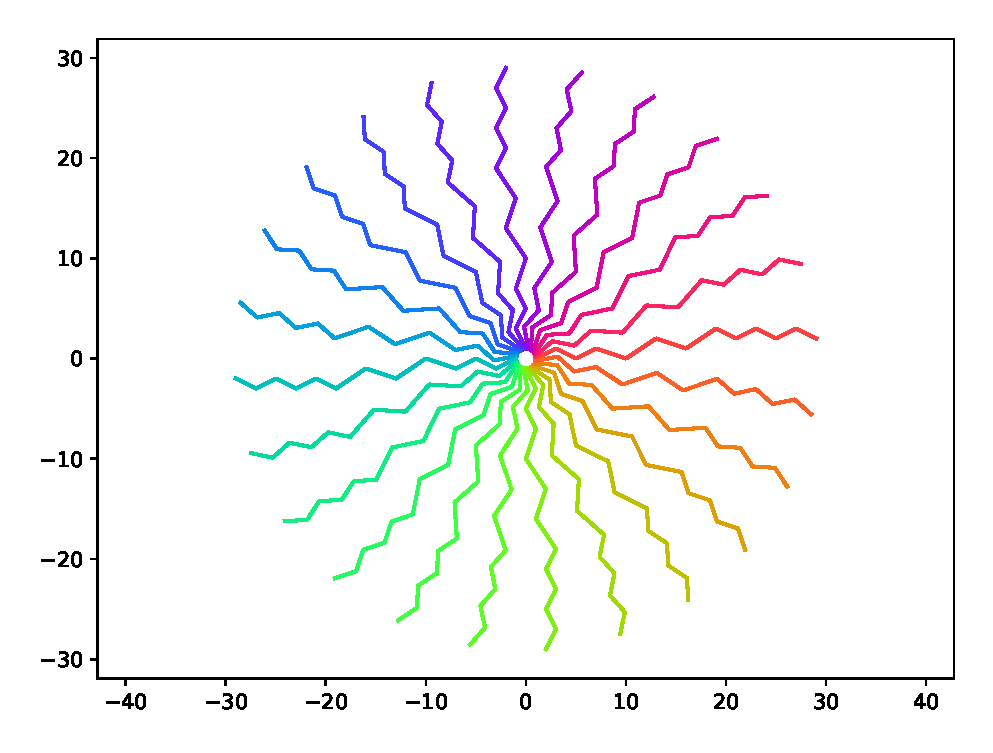
\epsfig{file=Rotated.eps, scale=0.7}
\caption{Creative Rotated Shape}
\end{center}
\end{figure}

\begin{figure}[htb!]
\begin{center}
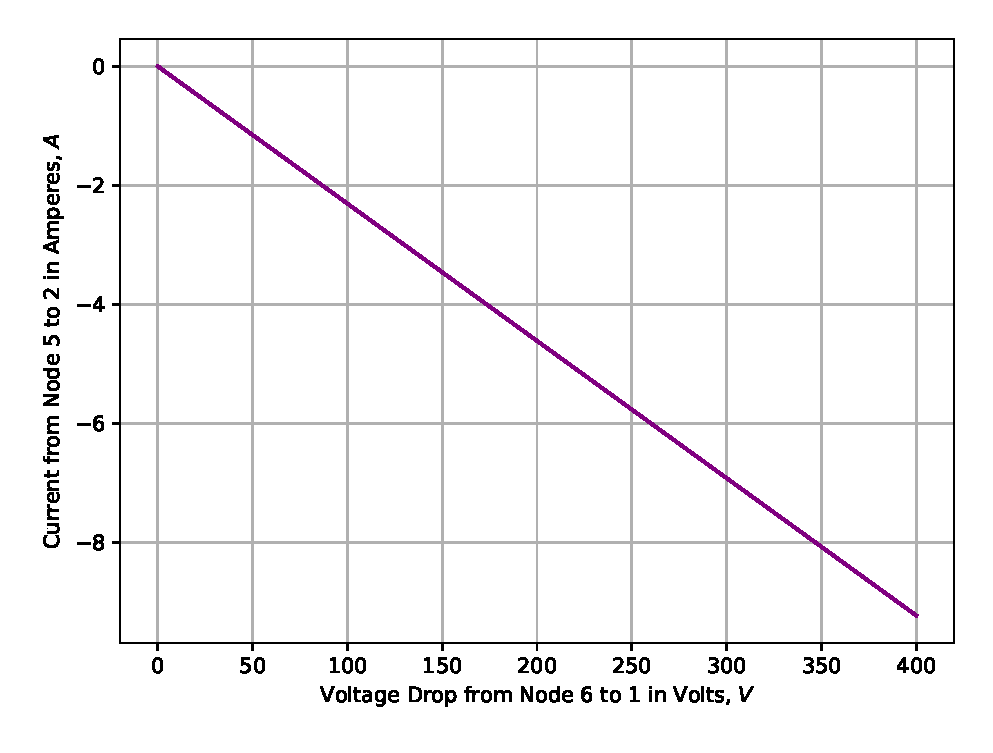
\epsfig{file=CurrentVoltage.eps, scale=0.7}
\caption{Current vs. Voltage}
\end{center}
\end{figure}

\begin{figure}[htb!]
\begin{center}
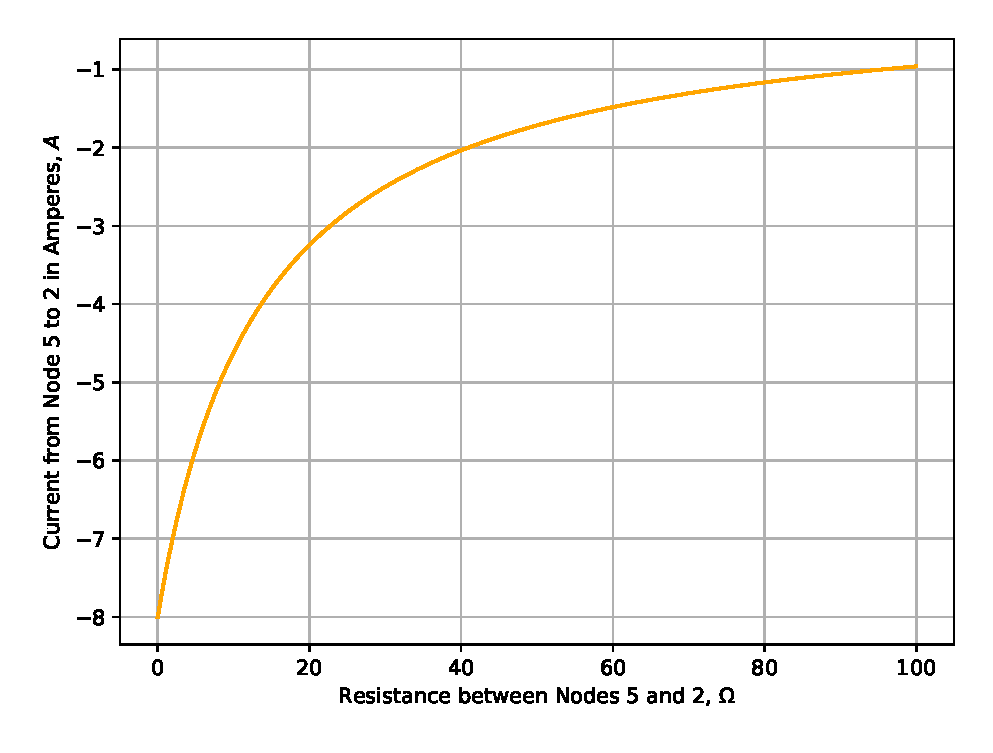
\epsfig{file=CurrentResist.eps, scale=0.7}
\caption{Current vs. Resistance}
\end{center}
\end{figure}

\begin{figure}[htb!]
\begin{center}
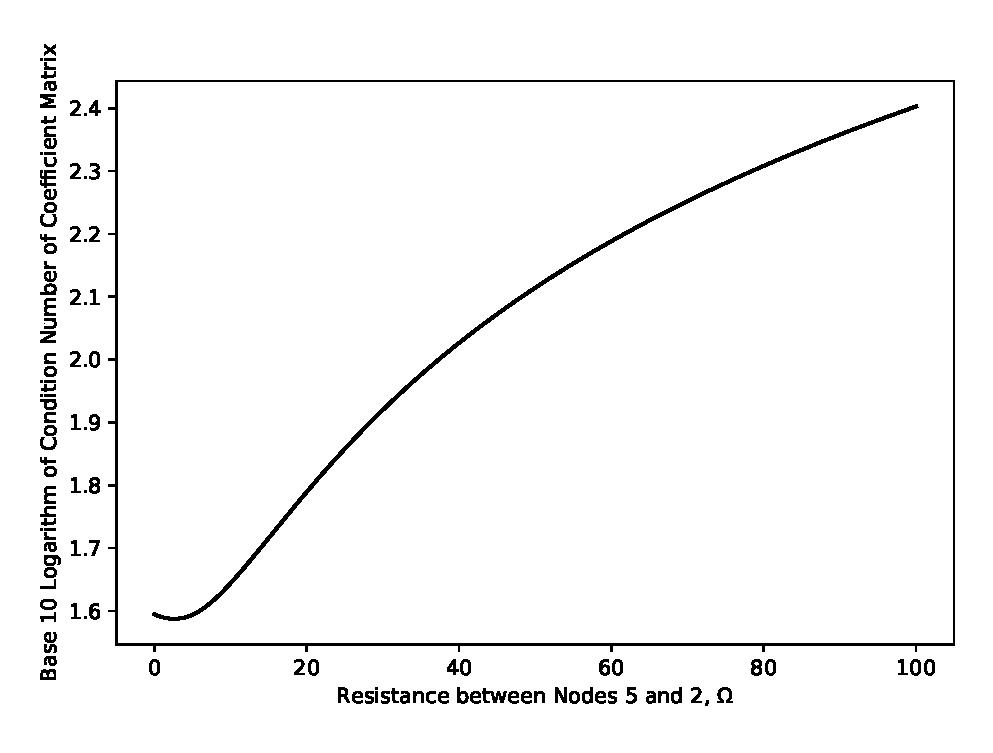
\epsfig{file=ConditionResist.eps, scale=0.7}
\caption{Condition Number vs. Resistance}
\end{center}
\end{figure}

\end{document}
